\chapter{Détection de la somnolence et l'hypovigilance en utilisant l'apprentissage profond}
\markboth{Détection de la somnolence et l'hypovigilance en utilisant l'apprentissage profond}{}


%-------------------
%-------------------
%-------------------

\section{Inroduction}
Les accidents de la route représentent une sérieuse menace pour la vie humaine, entraînant des pertes matérielles et humaines considérables, notamment en Algérie.
En 2022, les routes algériennes ont enregistré 22 980 accidents, causant 3 409 décès et 30 479 blessés\cite{AtlasMagasine2}, des chiffres alarmants qui montrent une tendance à la hausse constante.

Suite à des recherches et enquêtes menées par la DNSR, il a été établi que la somnolence est l'une des principales causes des accidents de la route. Selon la dernière étude du CNPSR en 2016 (DNSR avant) un tiers des accidents de la route en Algérie sont dus à la somnolence au volant. Cette situation a suscité des appels à classer les troubles du sommeil dans la même catégorie que les stupéfiants et l'alcool en raison de leur dangerosité\cite{autobip}.

En effet, sur les 10 accidents de la route enregistrés au cours des dix premiers mois de 2016, 2 500 ont été attribués à la somnolence au volant\cite{autobip}.

\section{Contexte et importance du problème}
La lutte contre la somnolence au volant revêt une importance cruciale, étant donné le nombre considérable d'accidents qu'elle entraîne, ainsi que les dégâts matériels et les pertes humaines qu'elle engendre. Selon des données fournies exclusivement pour le secteur de la Gendarmerie à la délégation nationale à la sécurité routière, le nombre d'accidents causés par la somnolence est en constante augmentation, comme le montre la \hyperlink{fig0} {figure}. Cette problématique est désormais classée dans la même catégorie que les stupéfiants et l’alcool en raison de sa dangerosité, non seulement en Algérie, mais à l’échelle mondiale. Par exemple en France, une étude de l'ASF en 2016 a identifié la somnolence au volant comme l’un des principaux facteurs de mortalité routière, comme illustré dans la \hyperlink{fig1} {figure 2}. Cette constatation démontre clairement que la détection de la somnolence a un impact potentiel sur la sécurité routière, où elle peut sauver des milliers de vies en restant vigilants et en s’arrêtant dès les premiers signes de fatigue, contribuant ainsi à réduire les risques d’accidents sur les routes en identifiant les signes de fatigue, ce qui permet de prendre des mesures pour éviter de conduire dans cet état dangereux.
\begin{figure}[H]
\hypertarget{fig0}{}
    \centering
    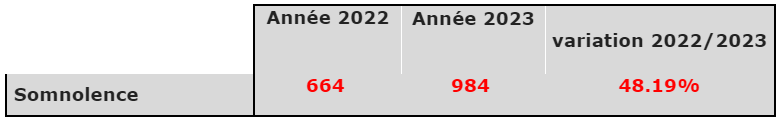
\includegraphics{img/accidents.png}
    \caption{ accidents corporels de la route causées par la somnolence}
    \label{fig:enter-label}
\end{figure}
\begin{figure}[H]
\hypertarget{fig1}{}
    \centering
    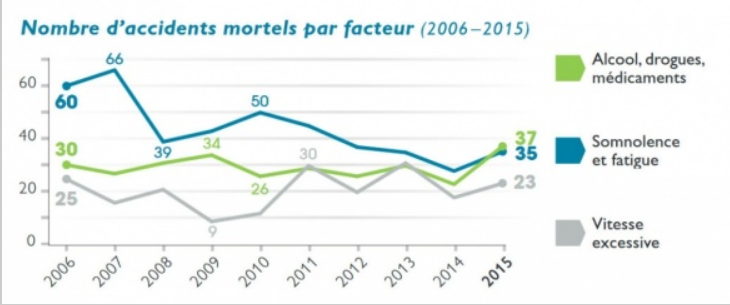
\includegraphics[]{img/frn.png}
    \caption{nombre d'accidents mortels par facture 2006-2015}
    
\end{figure}
Afin de mettre en place des mesures préventives efficaces, des systèmes de détection de la somnolence ont été développés. Ces systèmes ont pour objectif d'avertir les conducteurs avant que leur niveau de somnolence ne devienne critique, permettant ainsi de prévenir les accidents liés à ce phénomène. Néanmoins, la détection de la somnolence reste un défi majeur pour les chercheurs. Bien que de nombreux systèmes et solutions aient été développés, leur efficacité et leur fiabilité doivent encore être améliorées pour garantir une détection précise et prévenir efficacement les accidents.

\section{Somnolence au volant}
\subsection{La somnolence}
La somnolence, caractérisée par la tendance à s'endormir lorsque l'on souhaite rester éveillé, constitue l'un des symptômes les plus courants et significatifs signalés par les patients adressés à un spécialiste du sommeil. Ce phénomène est omniprésent et peut être le signe de diverses pathologies médicales, psychiatriques et troubles primaires du sommeil. Cependant, la somnolence est également un aspect physiologique, survenant au moins une fois par jour et pouvant être ressentie par tout individu dans des situations particulières\cite{haba2011somnolence}. Elle se manifeste souvent par des signes tels que des bâillements fréquents, une vision floue, des difficultés de concentration et une sensation de lourdeur dans les paupières. Plusieurs facteurs sous-jacents contribuent à cette sensation de somnolence. En conduisant, la somnolence peut conduire à des micro-sommeils, qui sont des périodes de sommeil de courte durée allant de 1 à 4 secondes\cite{somnolence}. Ces micro-sommeils peuvent considérablement compromettre la sécurité routière en réduisant la vigilance du conducteur et en augmentant le risque d'accidents.\\ \\
La somnolence peut être causée par plusieurs facteurs, notamment:
\begin{enumerate}
    \item Les affections médicales aiguës, telles que les troubles électrolytiques (par exemple, l'hyponatrémie ou l'hypomagnésémie), les traumatismes crâniens, l'hypothermie et les infections (par exemple, la mononucléose ou la méningite), peuvent servir de cause sous-jacente de la somnolence.
    \item  Les affections médicales chroniques, telles que le syndrome de fatigue chronique, la fibromyalgie, l'obésité, la dépression, l'anxiété, le diabète, les douleurs chroniques et l'hypothyroïdie, peuvent également contribuer à la somnolence.
    \item Les troubles du sommeil, tels que l'insomnie, l'apnée du sommeil, la narcolepsie, le syndrome des jambes sans repos ou le retard de phase de sommeil, sont également caractérisés par la somnolence.
    \item Plusieurs médicaments, notamment les antihistaminiques, les benzodiazépines, les hypnotiques, les opioïdes, les antidépresseurs, les anticonvulsivants et les antipsychotiques, peuvent précipiter la somnolence, notamment en cas de surdose médicamenteuse.
    \item L'intoxication alcoolique peut également provoquer de la somnolence.
\end{enumerate}



\section{Détection de la somnolence au volant}
Lorsque les conducteurs sont somnolents ou épuisés, cela entraîne des conséquences graves pour la sécurité routière. Toutefois, si les conducteurs somnolents sont alertés à temps, de nombreuses tragédies peuvent être évitées. Pour ce faire, plusieurs technologies de détection de la somnolence peuvent être utilisées, surveillant les niveaux de vigilance des conducteurs et déclenchant une alarme dès les premiers signes d'assoupissement. Ces technologies prennent en compte divers aspects, notamment les expressions faciales telles que les signes de la fatigue ou la fermeture des yeux, les mouvements de la tête et les bâillements, qui révèlent des indices essentiels sur l'état de somnolence. En outre, la détection de la somnolence tient compte à la fois de l'état physique des conducteurs et de la façon dont ils sont conduits.
Cependant,Il existe plusieurs types de techniques de détection de la somnolence, chacune utilisant différents indices pour identifier les signes de la somnolence chez le conducteur:
\begin{enumerate}
    \item les méthodes basées sur des signaux physiologiques
    \item les méthodes basées sur le comportement 
    \item les méthodes basées sur le véhicule
\end{enumerate}
\begin{figure}[H]
    
    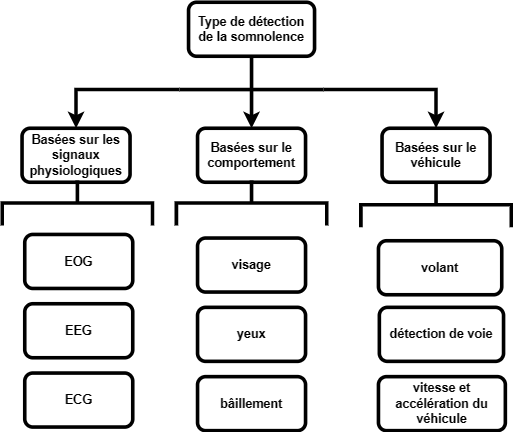
\includegraphics[]{img/indicateurs.drawio.png}
    \caption{ Types  de détection de la somnolence}
     \hypertarget{fig01}{}
\end{figure}
\subsection{Méthodes basées sur des signaux physiologiques}
Ce type de technique repose sur l'exploitation des signaux physiologiques associés à la réponse du corps à la fatigue, à l'aide de capteurs fixés sur le corps du conducteur. Elle utilise des données acquises à partir de capteurs physiologiques tels que l'électrooculographie (EOG), l'électrocardiographie (ECG), l'électroencéphalographie (EEG).

Un électroencéphalographie (EEG) est un examen qui permet de détecter l’activité électrique dans le cerveau à l’aide de petits disques métalliques (électrodes) fixés sur le cuir chevelu (la tête). Les cellules du cerveau transmettent des signaux électriques et sont toujours actives, même lorsque vous dormez. Des lignes ondulées tracent l’activité et sont enregistrées pendant l’EEG. Cet examen permet de diagnostiquer plusieurs troubles du cerveau, notamment l'état de vigilance et les troubles du sommeil\cite{EEG} .

Les chercheurs se concentrent souvent sur des bandes de fréquences telles que les ondes alpha, thêta et delta, où la bande delta (entre 0,5 et 4 Hz) indique l'activité de sommeil, la bande thêta (entre 4 et 8 Hz) indique la somnolence, et la bande alpha (entre 13 et 25 Hz) correspond à la vigilance. L'analyse de l'activité électrique du cerveau fournit des informations sur les états cognitifs et les niveaux de vigilance\cite{sahayadhas2012detecting}.
 
 \begin{figure}[H]
    \centering
    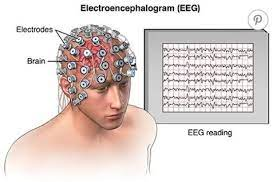
\includegraphics[]{img/EEG.jpg}
    \caption{Placement des électrodes EEG}
     
\end{figure}
L'électrocardiographie ECG est une technique qui repose sur la détection de l'activité électrique du cœur à l'aide d'électrodes placées sur le corps du conducteur. Cet enregistrement peut servir de marqueur potentiel pour prédire la somnolence ou la fatigue en se basant sur la variabilité de la fréquence cardiaque (VFC)\cite{abe2014development,zhang2012drowsiness} . La VFC est un indicateur du fonctionnement du système nerveux autonome (SNA), qui régule les activités cardiaques pour maintenir l'homéostasie du système cardiovasculaire. L'activité du SNA varie selon les périodes de stress, de fatigue et de somnolence. Pendant l'éveil, l'activité sympathique (AS) augmente et/ou l'activité parasympathique (APS) diminue, tandis que pendant la somnolence ou la fatigue, on observe une augmentation de l'APS ou une diminution de l'AS\cite{vicente2011detection}. Différentes méthodes temporelles et fréquentielles ont été utilisées pour analyser la VFC à partir des intervalles RR (IRR),où un IRR  représente le temps qui sépare le début de deux ondes R successives dans le tracé de l’ECG. Les variations de ces caractéristiques temporelles et fréquentielles de l'ECG peuvent fournir des indications sur l'état de somnolence.
 \begin{figure}[H]
    \centering
    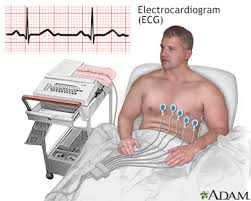
\includegraphics[]{img/ECG.jpg}
    \caption{Placement des électrodes ECG}
     
\end{figure}
L’électrooculographie (EOG) est une technique d’enregistrement des mouvements oculaires en utilisant des électrodes placées autour des yeux. Cette méthode permet de détecter et d’enregistrer les mouvements des yeux, tels que les clignements des yeux et les mouvements lents caractéristiques de la somnolence. En plaçant les électrodes autour des yeux.Le signal EOG identifie la somnolence en se basant sur les mouvements oculaires en mesurant le potentiel électrique entre la cornée et la rétine à partir du champ électrique qui reflète l'orientation de l'œil\cite{sahayadhas2012detecting}.l’EOG mesure les variations du potentiel électrique générées par les mouvements des muscles oculaires. Ces variations sont enregistrées sous forme de signaux électriques qui peuvent être analysés pour évaluer l’activité oculaire et détecter les signes de somnolence chez le conducteur.\\
%Les signaux physiologiques peuvent fournir une mesure précise de la somnolence car ils sont fortement corrélés avec la somnolence. Cependant, cela utilise des techniques invasives et peut rendre le conducteur inconfortable en raison de problèmes de portabilité et de faisabilité limitée\cite{mittal2016head,awais2017hybrid}.%
 

\subsection{Détection  basée  sur le véhicule }
Ce type de détection mesure le niveau de somnolence en fonction des capteurs embarqués dans le véhicule et recueille plusieurs métriques indicatives pour déterminer le niveau de vigilance/somnolence du conducteur grâce à ses comportements de conduite\cite{doudou2020driver}. Les trois principaux aspects de ce type incluent le mouvement du volant, la déviation et la position du véhicule, ainsi que la vitesse et l'accélération du véhicule. L'angle et la trajectoire du volant deviennent irréguliers, et la plage de déviation augmente significativement lorsqu'un conducteur est dans un état de somnolence\cite{dong2010driver,zhong2007localized} . Les approches utilisant la déviation et la position du véhicule reposent sur certaines métriques telles que l'écart-type de la position de la voie (SDLP), qui mesure la position du véhicule par rapport à la voie médiane de la route. Il a été démontré que le score KSS(score de somnolence de Karolinska ) du conducteur peut affecter le score SDLP car les deux sont étroitement liés. Par conséquent, plus le conducteur est somnolent, plus le score SDLP sera élevé, et le SDLP pourrait être un indicateur potentiel pour détecter la somnolence\cite{dong2010driver,chen2015identification,ingre2006subjective}. Enfin, la vitesse et l'accélération du véhicule peuvent indiquer une conduite anormale causée par la somnolence, car les conducteurs somnolents peuvent augmenter ou diminuer accidentellement l'accélération de leur véhicule\cite{doudou2020driver}. 

\subsection{Détection  basée sur le comportement}
Ce type de détection se focalise sur l'analyse des caractéristiques du visage telles que le clignement des yeux, le bâillement et la direction du regard sont capturées à l'aide d'un capteur intégré dans la voiture, puis observées pour détecter la somnolence\cite{vijayan2020comparative} . Les paramètres utilisés dans la détection de la somnolence comprennent le pourcentage de fermeture des yeux (PERCLOS), le rapport d'aspect de l'œil (EAR), le rapport d'aspect de la bouche (MAR) et la position de la tête. Le PERCLOS est le pourcentage du nombre total de trames où les yeux sont détectés comme fermés dans un intervalle de trame spécifique. Un seuil prédéterminé est défini afin de classifier si les yeux sont fermés ou ouverts. Ensuite, le PERCLOS est calculé sur la base de la zone approximative de l'iris pour identifier la somnolence du conducteur\cite{junaedi2018driver,zhang2017research} . Pendant ce temps, l'EAR est utilisé pour enregistrer la fréquence de clignotement des yeux en fonction de la proportion entre la hauteur et la largeur de l'œil\cite{maior2020real,you2019real2,soukupova2016eye} . La valeur EAR est presque constante lorsque l'œil est ouvert et tombe à zéro lorsque l'œil est fermé. Le MAR est similaire à l'EAR, mais il utilise davantage de repères de la bouche pour détecter les bâillements, et l'échelle est opposée à l'EAR. Plus la bouche est ouverte, plus la valeur de MAR sera grande\cite{houssaini2019real,mohanty2019design}. Le MAR peut être mesuré en fonction des régions de couleur rouge des lèvres. Cependant, la performance dépend encore fortement des conditions d'éclairage \cite{niloy2020brief}. Le changement de position de la tête est l'un des phénomènes de comportement typiques montrés par les conducteurs somnolents. Il est généralement observé chez les conducteurs au début de la somnolence, marqué par l'augmentation de la fréquence des inclinaisons de la tête vers l'arrière\cite{brandt2004affordable,dreissig2020driver} .

\subsection{ Comparaison entre les techniques de détection de somnolence }
\begin{table}[htbp]
    \centering
    \begin{tabularx}{\textwidth}{|X|X|X|X|}
    \hline
        techniques  & Mesures & avantages & Incovénients \\
        \hline
      basée sur le comportement& Fermeture des yeux et position de tête, bâillement et analyse de la bouche , l’expression faciale  &  Non-intrusifs, facile à utiliser & Dépend des conditions extérieures\\ 
      \hline
      basée sur me véhicule & Angle du volant, détection de voie et la vitesse de véhicule & Non-intrusifs & Conditions climatiques, l’état des routes, expérience de conducteur\\
      \hline
      basée sur les signaux physiologiques &  ECG, EOG, EEG & Détection anticipée, fiable & Intrusif, faible qualité de signal dans les solutions non-intrusives \\
\hline
    \end{tabularx}
    \caption{Comparaison entre les types des techniques de détection de somnolence}
    \label{tab:my_label}
\end{table}


Voici une version corrigée de votre texte :

Malgré la fiabilité des signaux physiologiques pour la détection de la somnolence, leur intrusivité réside dans la nécessité d'un équipement supplémentaire qui doit être attaché au corps du conducteur pour collecter les données permettant d'identifier son état. De même, les systèmes basés sur le véhicule, qui dépendent de plusieurs paramètres extérieurs, restent des indices difficiles à exploiter et peuvent perturber le conducteur. Cette limitation rend ces deux techniques inappropriées à mettre en œuvre en temps réel. Par conséquent, la plupart des études se concentrent sur la troisième catégorie, qui utilise les caractéristiques comportementales des conducteurs, car elles sont non invasives et impliquent la vision par ordinateur pour la détection de la somnolence. Les mesures comportementales, telles que les mouvements oculaires habituels, les expressions faciales, les bâillements et l'orientation de la tête, sont mesurées sans nécessiter l'ajout d'équipement supplémentaire, sauf une caméra pour capturer les images. En conséquence, l'analyse des caractéristiques comportementales est une solution rentable et facile à utiliser, mais elle reste un défi à améliorer pour une exploitation optimale étant donné la qualité des données acquises.

\section{Approches de détection de la somnolence}
% mena 

Étant donné que la détection de la somnolence basée sur le comportement du conducteur offre des solutions rentables et non intrusives ne nécessitant pas d'équipement supplémentaire, nous avons choisi de mener une recherche sur les solutions déjà adoptées dans ce domaine. Plus particulièrement, celles basées l'apprentissage profond et la vision par ordinateur, en commençant par présenter une étude comparative des travaux déjà réalisés basés sur ces technologies.\\
\begin{table}[htbp]
    \centering
    \begin{tabularx}{\textwidth}{|X|X|X|X|X|}
    \hline
       \textbf{Référence}  & \textbf{Jeu de données} & \textbf{Méthods}&\textbf{Meilleur résultat}& \textbf{Année}\\ \hline
       \cite{chirra2019deep} &Un ensemble de données privé comprend 2850 images & Deep-stacked CNN& Précision de 96,42\% & 2019 \\ \hline
      
        \cite{salman2021driver}&YawDD, qui se compose de 107 images & Ensemble CNN (ECNN) & Score F1 de 93 \%  & 2021\\ \hline
        \cite{rajkar2022driver} & Deux ensembles de données : le Closed Eye in the Wild (CEW) et le Yawing Detection Dataset (YawDD)& réseaux de neurones convolutifs (CNN) & précision de 96.86\% & 2022 \\ \hline
       \cite{Florez2023ACA}  &Ensemble de vidéos NITYMED & InceptionV3, VGG16 et ResNet50V2 &  Précision de 99,71 \% & 2023  \\ \hline
  
    \end{tabularx}
    \caption{Modèles de détection de la somnolence basés sur l'apprentissage profond }
    
    \label{tab:my_label}
\end{table}
\newpage
Dans l'étude \textbf{\cite{chirra2019deep}} ils ont proposé un systeme de détection de la somnolence du conducteur basé sur  l'état des yeux en utilisant l'apprentissage profond. La méthode de détection de visage Viola-Jones est utilisée pour reconnaître la région des yeux, un réseau de neurones convolutifs profonds empilés est créé pour déterminer les images clés importantes dans les séquences de caméra, et la couche SoftMax dans un classificateur CNN est utilisée pour classifier si le conducteur est endormi ou non.  Le travail proposé est évalué sur un ensemble de données collectées et montre une meilleure précision avec 96,42 \% par rapport au CNN traditionnel.\\ \\



Dans l’étude mentionnée dans \textbf{\cite{rajkar2022driver}}, les auteurs ont proposé un système basé sur deux modèles de réseaux de neurones convolutifs (CNN) pour identifier la somnolence du conducteur en utilisant la méthode de la cascade de HAAR pour la détection du visage et des yeux. Le premier modèle CNN a été entraîné et testé sur un ensemble de données CEW pour l'état des yeux, tandis que le deuxième a été entraîné et testé sur le jeu de données YawDD pour détecter l'état de la bouche, qu'elle soit fermée ou ouverte. Les deux modèles ont atteint une précision moyenne de 96,86 \%.\\ \\


Une autre étude \textbf{\cite{salman2021driver}} a proposé un système basé sur quatre techniques différentes de CNN appliquées à l'ensemble de données YawDD pour mesurer le degré de somnolence en fonction de la fréquence des bâillements, des poses spécifiques et des variations d'occlusion. Le réseau de neurones convolutifs ensembliste (ECNN) proposé a surpassé les approches traditionnelles basées sur les CNN, atteignant un impressionnant score F1 de 0,935. Les trois autres approches CNN (CNN1, CNN2 et CNN3) ont obtenu des scores F1 de 0,92, 0,90 et 0,912, respectivement.\\ \\


Dans l’étude mentionnée dans \cite{Florez2023ACA}, Florez et al. ont proposé un système de détection de la somnolence au volant via l’identification en temps réel de l’état des yeux en utilisant trois algorithmes d’apprentissage profond pré-entraînés, à savoir InceptionV3, VGG16 et ResNet50V2. À cet égard, ils ont utilisé l’ensemble de données appelé NITYMED pour l'entraînement, contenant des vidéos de conducteurs présentant divers états de somnolence, où les yeux ont été extraits après la conversion des vidéos en utilisant un algorithme basé sur l'exploitation des points de MediaPipe Mesh. Ce système a été testé sur une partie de test de la même dataset et a atteint une précision de 99,71 \%, marquée par le modèle ResNet50V2 pré-entraîné, démontrant ainsi son efficacité. %

% lahna 


\section{Jeux de données utlisés pour la détection de la somnolence}
\begin{enumerate}
    \item \textbf{YawDD}: est un ensemble de données de détection de l'ouverture de la bouche (ou du sommeil) qui comprend deux jeux de données vidéo de conducteurs avec différentes caractéristiques faciales. Les vidéos ont été recueillies en demandant à des candidats masculins et féminins de s'asseoir dans le siège du conducteur d'une voiture. Les vidéos ont été enregistrées dans des conditions d'éclairage réelles et variables. 
Le premier jeu de données comprend 322 vidéos, où une caméra est installée sous le rétroviseur avant du véhicule. Chaque participant dispose de trois ou quatre vidéos avec différentes conditions de bouche, telles que normale, parlant/chantant et ouvrant la bouche. 

Le deuxième jeu de données comprend 29 vidéos, où une caméra est installée sur le tableau de bord devant le conducteur. Chaque participant dispose d'une seule vidéo avec les mêmes conditions de bouche, toutes dans la même vidéo. Le véhicule était garé pour les deux jeux de données pour assurer la sécurité de l'environnement pour les participants\cite{inproceedings}.
\item \textbf{NITYMED}:Ce jeu de données comprend 130 vidéos capturées à Patras, en Grèce, mettant en scène des conducteurs dans de vraies voitures circulant dans des conditions nocturnes, où détecter la somnolence est particulièrement crucial. Les conducteurs participant à l'ensemble de données se composent de 11 hommes et de 10 femmes, chacun présentant diverses caractéristiques telles que la couleur des cheveux, la présence de barbe et de lunettes. Les vidéos sont divisées en deux catégories principales :

Bâillements : Ces vidéos montrent des conducteurs baillant trois fois par vidéo, chaque vidéo durant environ 15 à 25 secondes. Il y a 107 vidéos dans cette catégorie.

Microsommeils : Dans ces vidéos, les conducteurs s'adonnent à des activités telles que parler et regarder autour d'eux, ponctuées de moments de microsommeil. Chaque vidéo de cette catégorie dure environ 2 minutes, et il y en a 21 disponibles\cite{nitymed}.
\item \textbf{CEW}:  cet ensemble de données contient 2423 sujets, parmi lesquels 1192 sujets avec les deux yeux fermés ont été collectés directement sur Internet, et 1231 sujets avec les yeux ouverts ont été sélectionnés à partir de la base de données LFW\cite{CEW}.
\end{enumerate}
\section{Synthése}
D'après l'examen et la comparaison des travaux déjà existants dans le domaine de la détection de la somnolence , qui se base sur l'analyse du comportement des conducteurs et utilise l'apprentissage profond, nous constatons que la plupart de ces travaux ont opté pour l'utilisation des réseaux de neurones convolutifs (CNN) lors de la conception de leurs modèles. De plus, l'adoption de la notion d'apprentissage par transfert, en exploitant les connaissances des modèles pré-entraînés, ainsi que la combinaison de modèles, a nettement amélioré leurs performances et leur efficacité dans la détection de systèmes déjà existants dans ce domaine. Il est important de noter que le choix du jeu de données a également contribué à cette amélioration de performance et d'efficacité .

\section{l'analyse oculaire pour la détection de la somnolence }
Dans un monde où la fatigue au volant peut avoir des conséquences désastreuses, la technologie d'analyse oculaire associée à la détection de la somnolence représente une avancée significative pour la sécurité routière. Cette technologie innovante utilise des systèmes de suivi oculaire pour analyser les mouvements et les clignements des yeux, permettant ainsi de détecter les premiers signes de somnolence chez les conducteurs. Par exemple, en Europe, cette technologie existe déjà sous la forme d'une option dans les véhicules haut de gamme, appelée DMS (Driver Monitoring System), qui utilise l'intelligence artificielle pour détecter les signes d'endormissement grâce à une caméra embarquée qui filme le visage et détecte les yeux même à travers des lunettes de soleil et dans des conditions d'éclairage ou d'illumination défavorables. Le système est capable de détecter la fermeture ou l'ouverture de la pupille, la fréquence des clignements des yeux et la direction du regard, comme illustré dans la \hyperlink{figDMS}{figure}, afin d'analyser l'état de vigilance du conducteur et d'envoyer ensuite des messages d'avertissement appropriés. Malgré le potentiel de cette technique, elle ne sera implantée que sur les véhicules neufs en Europe\cite{DMS}.
\begin{figure}[htbp]
    \centering
    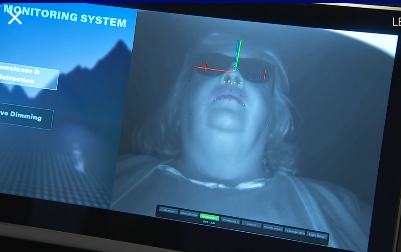
\includegraphics[width=0.5\textwidth ]{img/DMS.png}
    \caption{Driver Monitoring System }
    \hypertarget{figDMS}{}
    
\end{figure}
\subsection{Différence entre le globe oculaire et la région oculaire}
Le terme "oculaire" peut être lié à deux termes différents : "le globe oculaire" et "la région oculaire", qui peuvent être exploités différemment. Nous souhaitons clarifier la distinction entre ces deux termes, étant donné que notre étude se concentrera sur l'analyse de la région oculaire pour la détection de la somnolence.
\begin{enumerate}
    \item \textbf{Globe oculaire}\\
    le globe oculaire est un système (organe) important et interconnecté qui désigne toute la zone de l'œil, y compris le segment antérieur et postérieur de l'œil, et qui inclut généralement, mais sans s'y limiter, tous les tissus fonctionnels (par exemple, pour la vision) ou structuraux présents dans le globe oculaire, ainsi que les tissus ou les couches cellulaires qui tapissent en partie ou en totalité l'intérieur ou l'extérieur du globe oculaire. Les régions oculaires comprennent la chambre antérieur le cristallin, le nerf optique, la hambre postérieure, la cavité vitréenne, la choroïde, l'espace suprachoroïdien, l'espace sous-rétinien, la conjonctive, l'espace sous-conjonctival, l'espace épiscléral, l'espace intracornéen, l'espace épicornéen, la sclérotique, la pars plana, les régions avasculaires induites chirurgicalement, la macula et la rétine\cite{fedorchak2019thermoresponsive}. 
    \item \textbf{Région oculaire}\\
    D'une autre maniere, la région oculaire fait référence à la partie du visage qui contient l’œil et ses environs, tels que les cils, les paupières, les sourcils et la peau autour de l’œil\cite{Vizoni2020OcularRU}. 
\end{enumerate}



\begin{figure}[htbp]
    \centering
    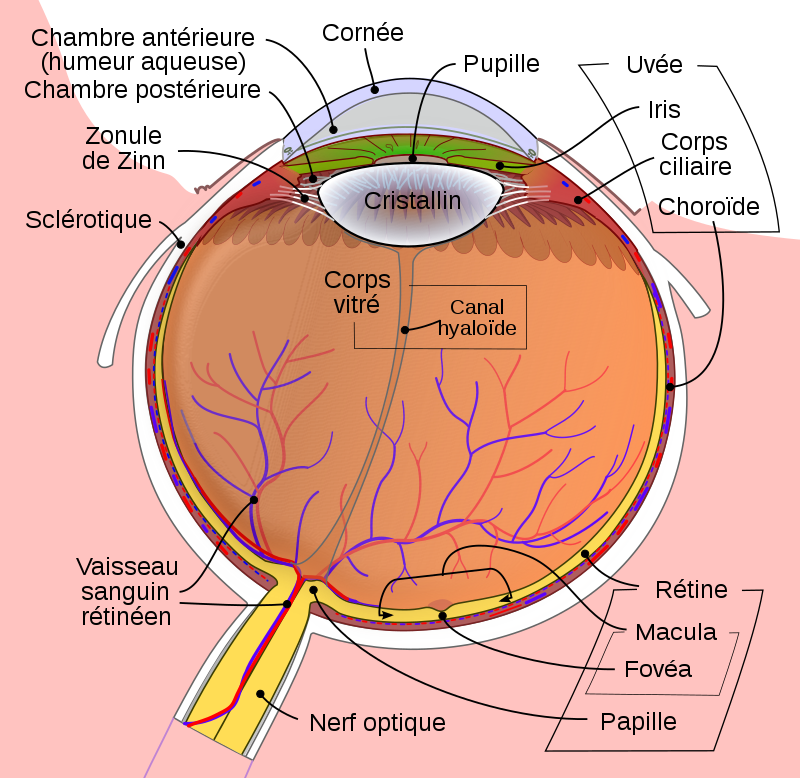
\includegraphics[width=0.5\textwidth ]{img/region_oculaire.png}
    \caption{globe oculaire }
    
\end{figure}
\begin{figure}[htbp]
    \centering
    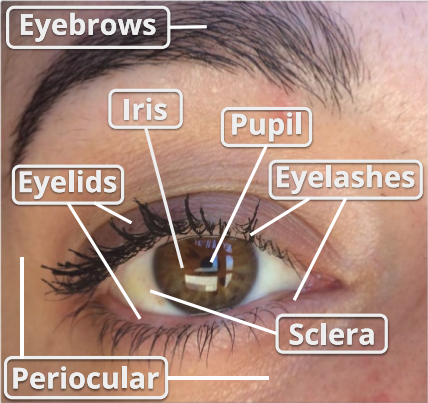
\includegraphics[width=0.5\textwidth ]{img/composants oculaire.png}
    \caption{région oculaire}

\end{figure}

\newpage


\subsection{Étapes de la reconnaissance oculaire}
 En général, la reconnaissance oculaire dédiée à la détection de la somnolence fonctionne selon ces étapes :

\begin{enumerate}
   \item \textbf{Acquisition de l'image}\\
    L'acquisition des données est une étape essentielle dans la reconnaissance oculaire. Les données sont collectées à partir de diverses sources telles que les caméras Pi Cam, les téléphones mobiles ou les caméras de surveillance.
   \item \textbf{Pré-traitement des données}\\
     Une fois que les données sont acquises, elles sont normalisées à une taille et un format spécialisés, puis subissent un pré-traitement afin de réduire le bruit et obtenir une bonne qualité d'image.
   \item \textbf{Détection de visage}\\
   L'étape suivante consiste à localiser le visage dans l'image, dans le but de faciliter la détection de la région oculaire, et ainsi éliminer les parties non pertinentes de l'image.
   \item \textbf{Détection de la région oculaire}\\
   Une fois que le visage est détecté à partir de l'image, il faut ensuite détecter la région d'intérêt qui contient les parties nécessaires de la région oculaire, puis l'identifier et l'isoler.
   \item \textbf{Amélioration de la résolution}\\
   Après la détection de la région de l’œil, l'étape suivante consiste à améliorer la résolution de l'image. Cette étape est appliquée lorsque la qualité de l'image est basse ou lorsque le nombre de pixels est limité.
   \item \textbf{Prétraitement (Alignement du centre de l'œil)}\\
   Après l'amélioration de la résolution de l'image, celle-ci est prétraitée pour aligner le centre de l’œil, ce qui implique d'ajuster l'image pour que le centre de la pupille soit positionné au milieu de l’image. Cela permet ensuite de détecter et d’isoler les parties pertinentes de la région oculaire, telles que l’iris ou la région périoculaire.
   \item \textbf{Extraction des caractéristiques}\\
   Cette étape consiste à identifier et extraire les caractéristiques distinctives de la région oculaire. Cela peut inclure l’analyse des motifs uniques de l’iris, la forme de l’œil et d’autres caractéristiques périoculaires.
   \item \textbf{Comparaison et correspondance}\\
   Enfin, cette étape consiste à comparer les caractéristiques extraites à une base de données de motifs oculaires connus pour trouver une correspondance.
\end{enumerate}



\begin{figure}[htbp]
    \centering
    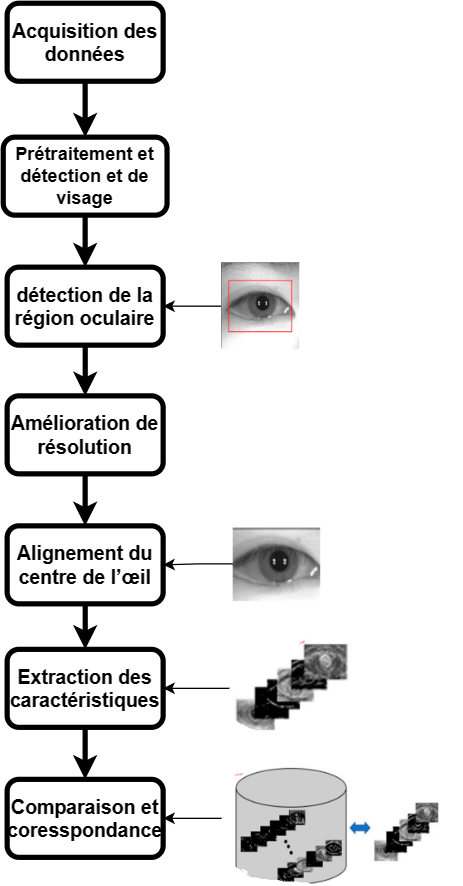
\includegraphics[width=0.5\textwidth ]{img/Diagramme sans nom.drawio.png}
    \caption{étapes de la reconnaissance oculaire}

\end{figure}

\subsection{Autre applications de l'analyse oculaire}
L'analyse oculaire peut non seulement être utilisée dans la détection de la somnolence, mais elle peut etre employé dans d'autres applications dans divers domaines et contextes. Les plus célèbres sont :
\begin{enumerate}
    \item \textbf{L'authentification biométrique}:L’analyse oculaire peut en effet servir à l’identification et la vérification des individus en utilisant les caractéristiques distinctives de leurs yeux. Les principales caractéristiques exploitées sont l’iris, la rétine et la région périoculaire (autour des yeux). Chacune de ces caractéristiques présente des motifs uniques qui peuvent être capturés et analysés pour l’identification.
    \item \textbf{Contrôle d'accès et sécurité }:L’analyse oculaire, attribuée à la reconnaissance oculaire, offre un haut niveau de précision pour distinguer les individus. Cela en fait un outil efficace à adopter dans divers systèmes de sécurité pour la vérification de l’identité, le contrôle d’accès et la surveillance. De même, certains smartphones intègrent la reconnaissance de l’iris pour offrir un déverrouillage sécurisé des appareils mobiles, assurant ainsi la protection des données personnelles et la confidentialité des utilisateurs.
    \item \textbf{Applications médicales et de santé }:Dans le domaine des applications médicales et de santé, les images oculaires sont largement utilisées à des fins diagnostiques et de suivi des maladies oculaires. De plus, la télémédecine bénéficie de la vérification de l'identité des patients lors de consultations à distance, améliorant ainsi l'accessibilité et la qualité des soins.
    \item \textbf{surveillance des conducteurs} :  elle joue un rôle important dans la surveillance des conducteurs, en identifiant les indices de somnolence ou d’inattention et la fatigue,  contribuant ainsi à la sécurité routière.
\end{enumerate}
\section{conclusion}
Durant ce chapitre, nous avons présenté les différents indices les plus utilisés dans les techniques de détection de la somnolence, en mettant en évidence leurs avantages et inconvénients. Nous avons également choisi de présenter des solutions axées sur le comportement du conducteur, notamment celles basées sur l’apprentissage profond, compte tenu de leurs performances remarquables. Nous avons examiné l’impact de l’apprentissage par transfert et de l’apprentissage ensembliste sur l’amélioration des résultats dans la détection de la somnolence. De plus, nous avons mentionné les jeux de données les plus utilisés par ces solutions. Enfin, nous avons défini la reconnaissance oculaire, en détaillant ses étapes et ses applications.












